% !TEX root = ../my-thesis.tex
%

\chapter*{Introduction}
\label{sec:introduction}

\cleanchapterquote{Un petit chapitre pour le doctorant, un grand chapitre pour l'humanité}{Doctorant anonyme}{(Citation temporaire)}

Cette thèse s'inscrit dans le cadre du traitement d'images médicales. Celle-ci est avant tout une thèse d'analyse d'images avec une teinte de biologie puisque les problématiques rencontrées durant celle-ci découlent directement de considérations anatomiques.

Le sujet de cette thèse est l'analyse de filtres de rehaussements de vaisseaux sanguins pour l'imagerie médicale 3D. L'objectif initial était de comparer ces filtres pour concevoir des outils de segmentation à destination de l'imagerie 3D du foie. Cet objectif a ensuite évolué pour se concentrer sur le développement d'outils d'analyses et d'évaluations de filtres de rehaussement de vaisseaux dans un cadre reproductible. En effet, ces filtres constituent une brique essentielle de la segmentation, mais peu de travaux portent sur leur évaluation de manière isolée.

Dans cette introduction, nous décrivons le contexte global de la thèse ainsi que ses principaux apports.

\section{Contexte global}
% quelques chiffres pour saisir l'importance du foie


Le foie est un des organes les plus importants du corps humain. Celui-ci participe à de nombreuses fonctions vitales comme la digestion, l'élimination des déchets ou la gestion de la glycémie. Les maladies liées au foie sont responsables de deux millions de morts par ans \cite{Asrani2019_liver_deseases}. On estime en effet à un million le nombre de morts par complications dû à la cirrhose, une maladie liée à l'apparition de tissus fibreux dans le foie. Un second million de décès est lié à une inflammation aigüe ou chronique du foie, l'hépatite, ainsi qu'au cancer du foie (carcinome). La cirrhose et du cancer du foie sont les $11^{ème}$ et $16^{ème}$ causes de mort à travers le monde. Deux de ces pathologies, la cirrhose et l'hépatite chronique, sont le plus souvent liées à une consommation régulière d'alcool. 
Dans ce contexte, le diagnostic et le suivi des maladies du foie est un objectif crucial pour les médecins. Les techniques d'imageries non invasives ont considérablement révolutionné ces deux tâches en permettant d'observer l'intérieur des patients sans nécessiter de chirurgie. Pour le foie, deux types d'imagerie sont particulièrement utilisés, la tomodensitométrie (TDM) et l'imagerie par résonance magnétique (IRM). La tomodensitométrie, inventée par Hounsfield en 1972 permet de mesurer l'absorption de rayons X par les tissus du patient. Cette acquisition se fait par coupes successives et permet de reconstituer de manière numérique une représentation 3D des organes. L'IRM est basée sur un principe similaire, mais repose sur l'utilisation d'un champ magnétique. Lors d'une IRM, on mesure le temps de précession des tissus, c'est-à-dire le temps de changement de leur orientation magnétique après une exposition brève et intense à un champ magnétique. Cette mesure permet ensuite de reconstituer un volume 3D des organes. La première machine IRM permettant l'acquisition d'un corps humain est développée en 1977 par Damasian. Pour les deux modalités, il est nécessaire dans certains cas d'utiliser un agent de contraste afin de différencier les tissus. C'est typiquement le cas pour les vaisseaux sanguins. 
Des agents de contraste, permettant de faire ressortir des tissus habituellement invisibles ou pauvrement contrastés, peuvent être utilisés pour les deux modalités (la pratique est cependant bien plus courante en IRM). Pour la tomodensitométrie, on utilise des agents à base d'iode ainsi que des agents à base de gadolinium pour l'IRM. L'agent est injecté par intraveineuse ce qui ajoute une difficulté supplémentaire lors de l'acquisition des images. En effet, le radiologue doit estimer correctement le temps de propagation du produit de contraste. Si l'image est acquise trop tôt, l'agent de contraste n'a pas le temps de se répandre dans le réseau vasculaire. Si l'image est acquise trop tard, l'agent de contraste se répand dans la totalité de l'organe rendant toute visualisation des vaisseaux impossible. En IRM, on prend en général plusieurs acquisitions (avant, pendant et après) de manière à donner un maximum d'informations au radiologue.
Les deux techniques d'imagerie sont complémentaires. La tomodensitométrie offre une grande résolution spatiale et permet de visualiser plus finement les détails, mais elle souffre d'un contraste entre les tissus plus faible. Au contraire, l'IRM possède une plus grande résolution de contraste, mais avec une résolution spatiale limitée. C'est le médecin radiologue qui a la charge de choisir la méthode la plus appropriée. Pour les vaisseaux du foie, les deux systèmes sont utilisés. Cependant, la doctrine médicale est d'exposer le moins possible un patient à un examen à risque, tel que le rayonnement ionisant émis par la tomodensitométrie. Il y a donc une utilisation croissante de la tomodensitométrie à faible dose de rayons X et de l'IRM, moins agressive que la tomodensitométrie. En contrepartie, l'extraction automatique des vaisseaux pour visualiser les réseaux vasculaires nécessite des algorithmes de plus en plus performants.


\section{Objectifs initiaux et projet ANR}
\label{sec:introduction:objectifs}
% Présentation du projet ANR

Cette thèse a été proposée dans le cadre du projet R-Vessel-X lancé en janvier 2019. Le projet est porté par Antoine Vacavant de l'institut Pascal en Auvergne Rhône-Alpe. R-Vessel-X a pour objectif l'extraction de vaisseaux sanguins du foie dans les images biomédicales. Un point clé du projet est de proposer des algorithmes robustes. Cette notion de robustesse est à prendre au sens large et regroupe :

\begin{itemize}
\item La solidité des modèles utilisés pour représenter et extraire les vaisseaux face à des changements de tailles, de formes ou d'intensités.
\item La fidélité des segmentations par rapport aux données originales et la possibilité de corriger celles-ci par les médecins.
\item La validation des solutions développées grâce à des mesures effectuées sur des données synthétiques, cliniques et un retour de médecins.
\item La dissémination des algorithmes et des données du projet afin d'assurer une pérennité de ces travaux et une réutilisation par la communauté.
\end{itemize}

Le projet R-Vessel-X rassemble quatre laboratoires de traitement d'images pour travailler sur ces thématiques (Fig. \ref{fig:labs}). Chaque laboratoire se différencie par une expérience particulière. Le LIRIS de l'université de Lyon et le LORIA de l'université de Lorraine apportent leur expertise sur l'analyse d'image par géométrie discrète et contribuent à développer la recherche reproductible. Le CReSTIC de Reims est spécialisé dans l'analyse d'images médicales, la simulation et la visualisation 3D. Enfin, l'institut Pascal de Clermont-Ferrand apporte son expertise sur l'analyse et la segmentation des vaisseaux sanguins du foie.

Afin de juger de la qualité des algorithmes de segmentation, et en particulier leur adéquation avec une utilité clinique, deux radiologues du CHU de Clermont-Ferrand ont rejoint le projet. Ceux-ci sont aussi en charge de la collecte des données nécessaires au projet.

L'entreprise Kitware Inc. est spécialisée dans le développement d'outils algorithmiques et de visualisation pour l'imagerie médicale. Elle propose ainsi plusieurs outils open sources tels que l'aide à la compilation CMAKE, la librairie de traitement d'images médicales ITK, la librairie de visualisation 3D VTK ou encore la plateforme de visualisation Girder. Deux ingénieurs, issues de la branche Kitware de Lyon, participent à la dissémination du projet en intégrant les algorithmes développés aux outils existants de l'entreprise. Cette intégration passe en particulier par l'intégration d'un plug-in d'annotation et d'extraction des vaisseaux au logiciel de visualisation 3DSlicer. Cet outil open source permet d'assurer une visibilité et surtout une utilisation internationale des algorithmes du projet.

\begin{figure}[ht]
    \centering
    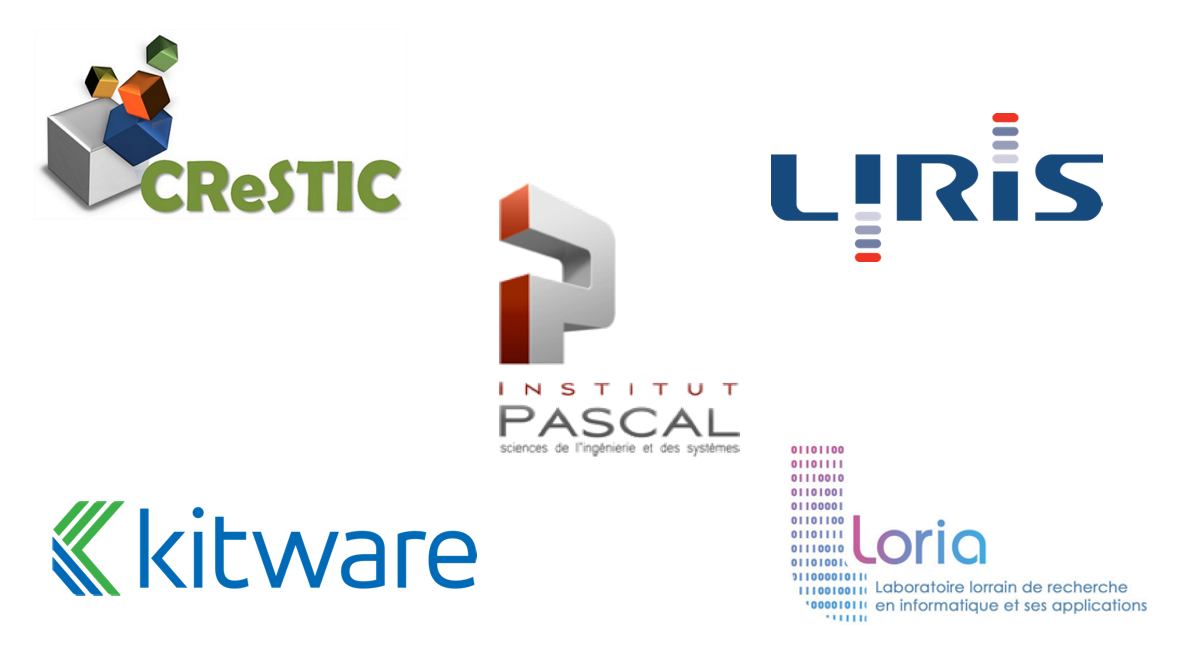
\includegraphics[height=4cm]{Images/labs.png}
    \caption{Structures participant au projet ANR R-Vessel-X}
    \label{fig:labs}
  \end{figure}

% Apports de la thèse
\section{Résumé de la thèse et apports}
\label{sec:introduction:résumé}

Cette thèse est encadrée par Bertrand Kerautret, professeur au LIRIS et Nicolas Passat professeur au CReSTIC. Elle est co-encadrée par Odyssée Merveille, maître de conférences du laboratoire d'imagerie médicale CREATIS qui  est rattaché à l'université et l'INSA de Lyon. L'objectif initial de cette thèse était la segmentation des vaisseaux du foie dans des images 3D. La segmentation des vaisseaux sanguins dans cet organe reste un problème ouvert que ce soit en IRM ou en TDM. En effet, les vaisseaux hépatiques sont des structures dont le nombre de voxels est faible par rapport à l'ensemble de l'image. Ils sont de plus difficilement identifiables par leur apparence bruitée et faiblement contrastée en plus d'être des structures fines, dont la taille peut approcher les limites de la résolution des images.

Un premier objectif a donc été d'identifier un ensemble de méthodes d'extraction existantes capables d'être efficaces dans ce contexte difficile. La famille des filtres de rehaussement de vaisseaux, semblait apporter une réponse à la plupart de nos problématiques. Ces filtres interviennent en amont de la segmentation. Ils permettent notamment de faire ressortir les structures tubulaires, et donc les vaisseaux, dans des contextes variés (Fig. \ref{fig:enhancement_example}). La littérature concernant ces filtres est plutôt variée avec une dizaine de filtres proposant des solutions complémentaires aux problématiques de la détection des vaisseaux sanguins. Pourtant, une analyse plus fine de la littérature montre qu'en pratique, la plupart des chaines de segmentation utilisent l'un des premiers filtres proposés dans la littérature : le filtre de Frangi \cite{Frangi1998_vesselness}. De plus, dans la plupart des articles, ce filtre est utilisé avec ses paramètres par défaut suggéré par Frangi en 1998, sans étudier si cette paramétrisation est idéale pour la tâche concernée.

\begin{figure}
% Frangi
\centering
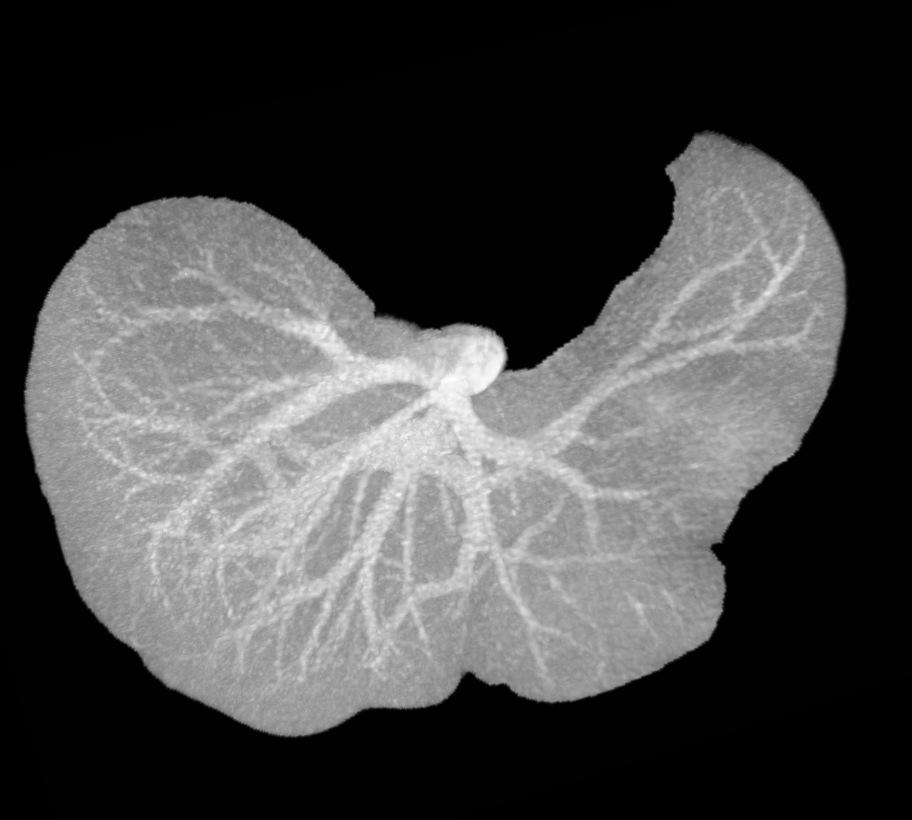
\includegraphics[clip = true, trim  =  10 60 10 60, height=25mm,width=36mm]{Images/Ircad_original_volume.png}
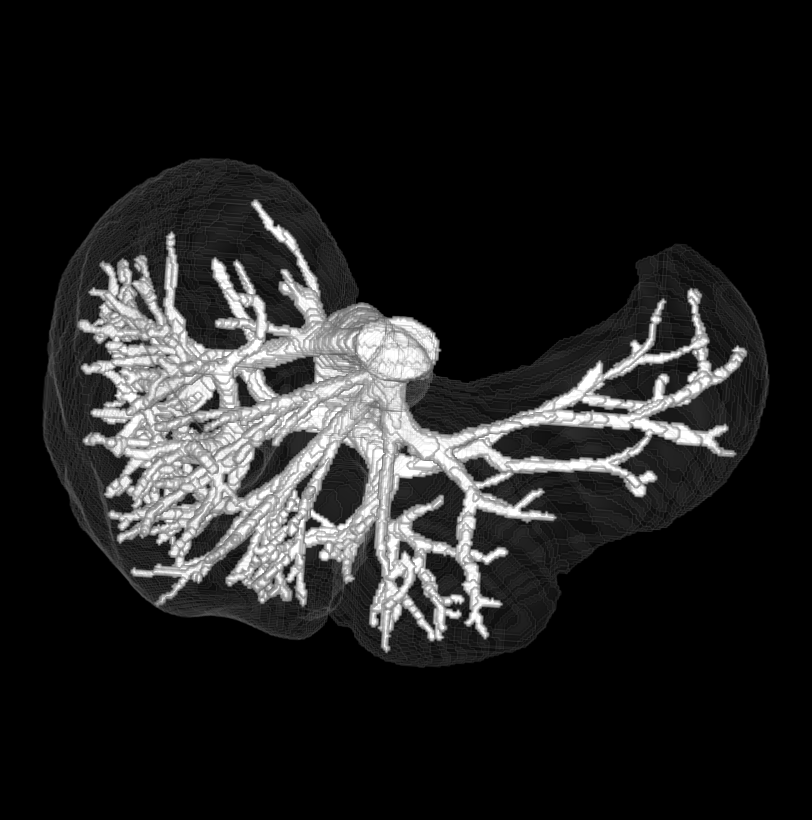
\includegraphics[clip = true, trim  =  10 150 10 150, height=25mm,width=36mm]{Images/Ircad_GT.png}
\\
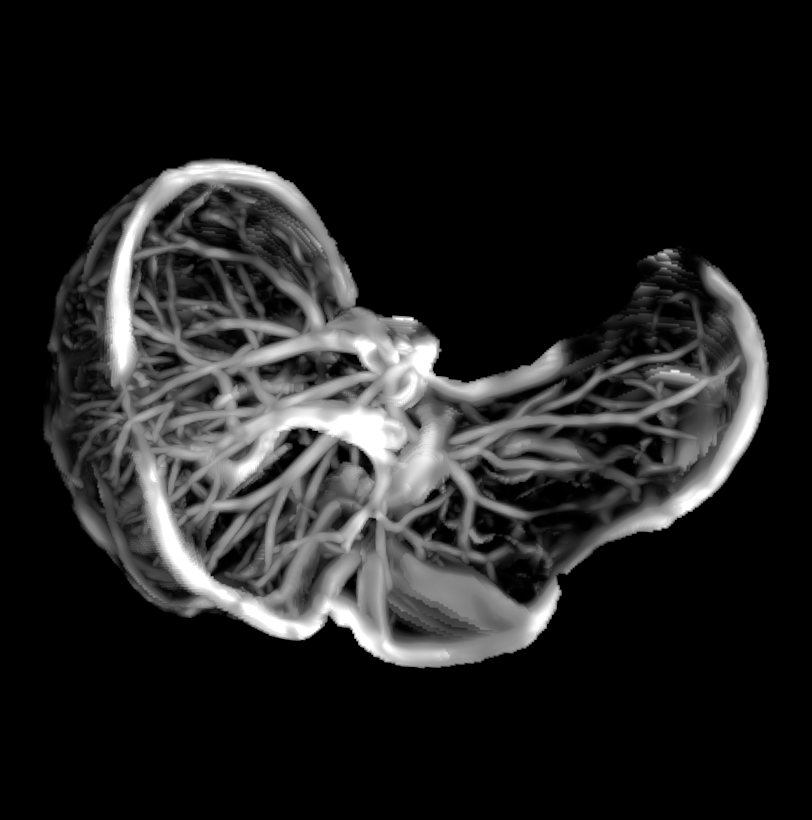
\includegraphics[clip = true, trim  =  10 150 10 150, height=25mm,width=36mm]{Images/Ircad_Frangi.png}
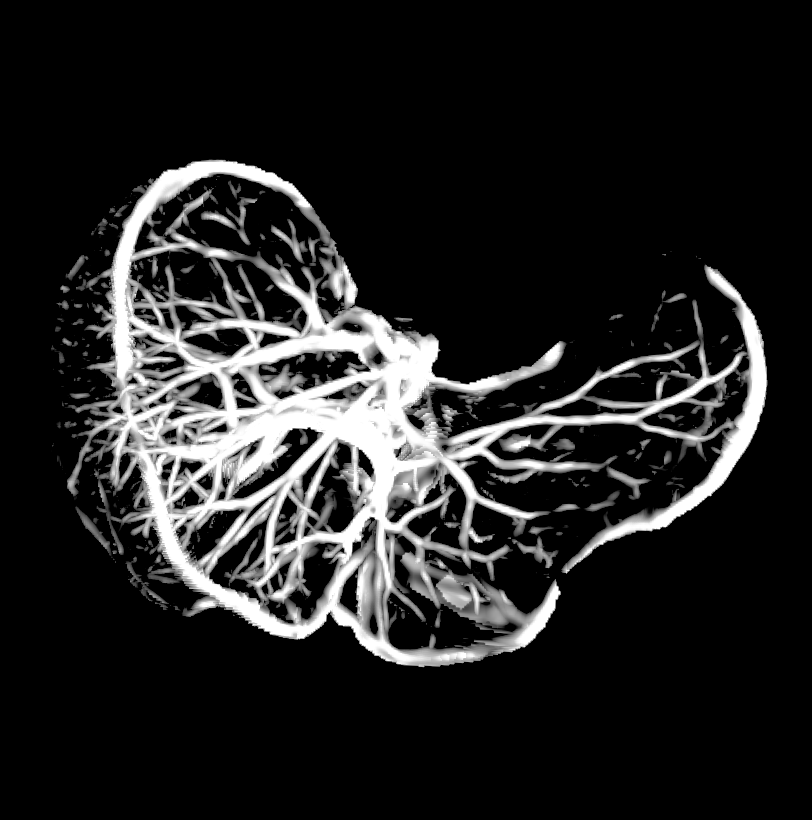
\includegraphics[clip = true, trim  =  10 150 10 150, height=25mm,width=36mm]{Images/Ircad_Jerman.png}
\caption{Image originale, Vérité terrain et différents filtres de rehaussement (Frangi et Jerman)}
\label{fig:enhancement_example}
\end{figure}

On peut donc légitimement se poser plusieurs questions. Le filtre de Frangi est-il le filtre le mieux adapté pour toutes les tâches de rehaussement de vaisseaux ? Est-ce qu'un filtre est plus adapté à une modalité particulière ? Les filtres plus récents proposent-ils un rehaussement de meilleure qualité ? Quel est l'impact réel de la paramétrisation des filtres sur le rehaussement final ?

Malheureusement, les bancs de tests considérant la seule qualité du rehaussement de vaisseaux sont peu nombreux et non extensibles. Leurs travaux ne peuvent donc pas être repris, soit parce que le code original n'est pas disponible, soit parce que les données ne sont pas publiques ou les deux en même temps. Dans l'esprit de robustesse du projet R-Vessel-X nous avons proposé les contributions suivantes :

\begin{itemize}
\item La collecte, l'implémentation et la mise à jour en C++ d'une sélection de filtres de rehaussement parmi les méthodes développées ces 20 dernières années. Chaque filtre illustre une réponse à une problématique distincte du rehaussement de vaisseau.
\item Un outil de comparaison de méthodes de rehaussement modulable permettant de comparer le rehaussement dans des zones spécifiques définies par l'utilisateur.
\item Une analyse quantitative poussée de ces filtres en fonction de la hiérarchie des vaisseaux définie par leurs tailles et leurs jonctions.
\item Une analyse qualitative liant le choix des paramètres des méthodes à la réponse théorique des filtres et leur impact sur le rehaussement.
\item Une démonstration en ligne permettant de tester les filtres et leurs paramètres sans installation préalable et sur ses propres données.
\item Un outil d'annotation spécialisé pour la segmentation du foie, ainsi qu'une série de bases de données publiques retravaillées pour répondre à un manque de données annotées. 
\end{itemize}

Ce travail a été réalisé dans un esprit de partage pour la communauté. C'est pourquoi une attention particulière a été apportée pour que ces travaux puissent être réutilisés et étendus par d'autres chercheurs, afin que ceux-ci n'ai pas à commencer leurs expériences à partir de zéro.

Ce manuscrit est organisé en 6 Chapitres : Le chapitre 1 présente le contexte médical de cette thèse. Celui-ci détaille l'anatomie du foie et présente les deux méthodes principales pour acquérir des images non invasives ainsi que les différents artefacts liés à cette acquisition. Le chapitre 2 présente le contexte scientifique en exposant de quelle manière la segmentation des vaisseaux est nécessaire à la visualisation des données. Nous présentons ensuite l'intérêt du rehaussement de vaisseaux pour la segmentation, ainsi que les concepts sur lesquels il se repose. Cette présentation s'effectue en deux temps avec l'introduction des espaces multi-échelles puis des caractéristiques de tubularité. Les espaces multi-échelles permettent de capturer les structures de l'image de différentes tailles, tandis que la caractérisation de la tubularité permet de ne sélectionner que les vaisseaux. Le chapitre 3 précise les choix effectués pour l'élaboration d'un banc de test afin d'évaluer les filtres de rehaussement. Ce chapitre décrit aussi les traitements des jeux de données nécessaires afin de permettre une analyse par zones d'intérêts du rehaussement. Le chapitre 4 illustre l'utilisation de ce banc de test avec une analyse des performances de 7 filtres de rehaussements à travers 5 jeux de données différents (TDM, IRM et 3 jeux d'IRM synthétique). Cette analyse étudie à la fois les performances des filtres les uns par rapport aux autres, mais aussi l'influence de leur paramétrisation sur le résultat final de manière quantitative et qualitative. L'évaluation est menée à la fois sur le rehaussement pris au niveau de l'organe, sur le voisinage des vaisseaux de différentes tailles et sur leurs bifurcations. Nous discutons ensuite dans le Chapitre 5 de la reproductibilité de nos travaux ainsi que du travail mené pour promouvoir leur diffusion. Cette diffusion passe par la promotion de nos travaux par des publications de journal et de conférences, mais aussi par le développement de démonstrateurs et de Plug-In pour un logiciel de visualisation 3D. Enfin le Chapitre 6, propose un bilan ainsi que des perspectives liées à ces travaux. Nous montrons en particulier, l'intérêt du rehaussement pour les méthodes de segmentations populaires actuellement. Nous explorons la possibilité de baser la segmentation des vaisseaux avec seulement l'annotation des bifurcations. 